
\chapter{Experimental Method}
\label{chap:experimental_method}


\section{Development of Linear Motion Platform}
\label{sec:development_of_linear_motion_platform}

A robotic linear motion platform was developed using Lego\textsuperscript{\textregistered} Mindstorms\textsuperscript{\textregistered} parts.
The platform was designed to carry a Lytro camera and a Nikon D5100 DSLR camera side-by-side as close as possible, with support for both cameras made out of Lego parts.
The motion platform consisted of a wheeled based that carried the cameras attached by a sewing thread to a drum, driven by two Mindstorms motors.
The drum was manually held in place during operation, and the Matlab RWHT NXT Toolbox \cite{rwth2007toolbox} was used to interface with the motors.

The angular velocity of the drum was manually calibrated using a stopwatch and ruler, allowing a desired velocity and linear distance to set in software.
Figure \ref{fig:motion_platform} shows the design of the linear motion platform.

\begin{figure}[h]
\centering
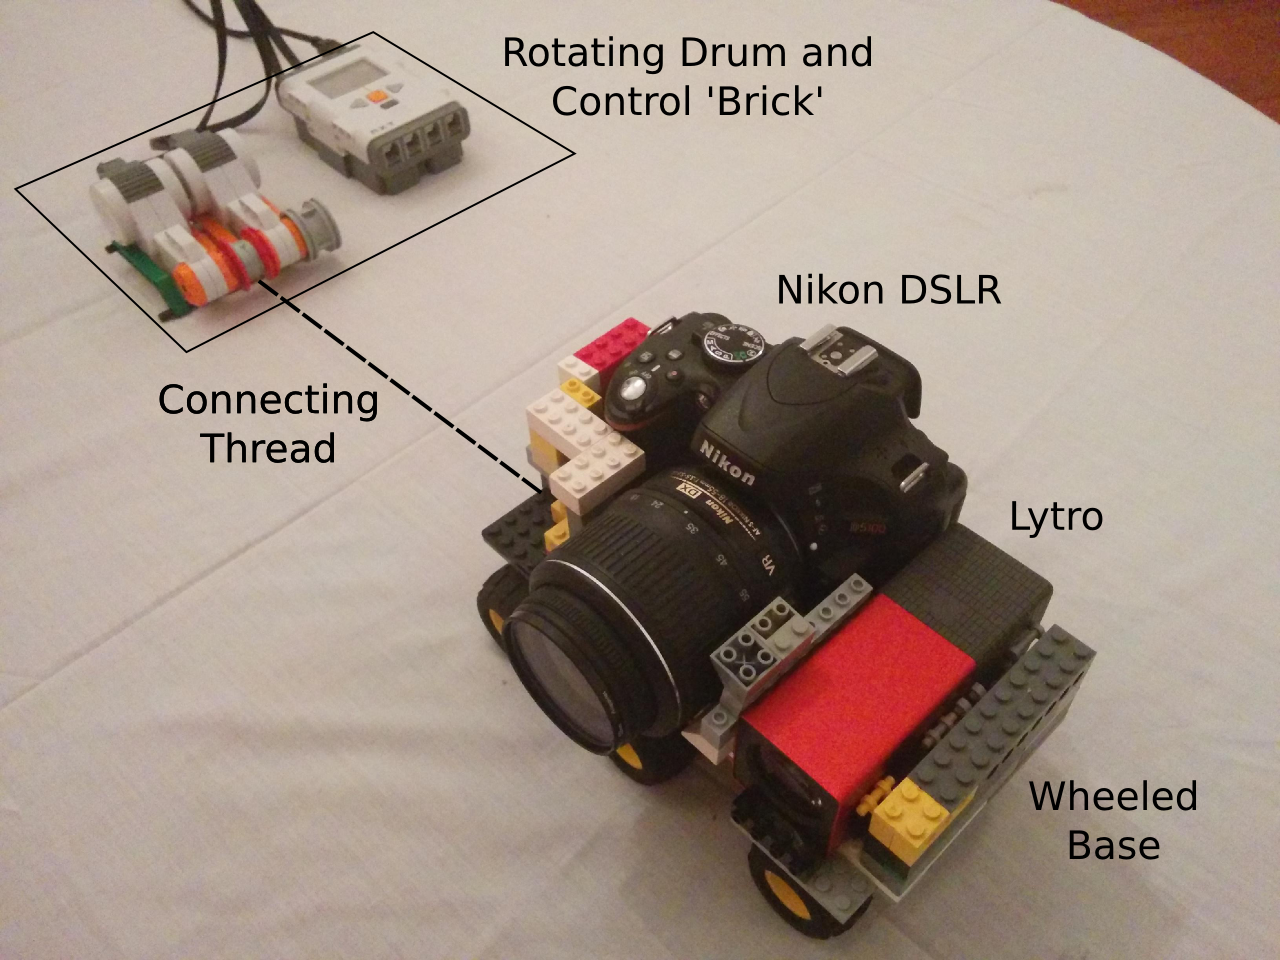
\includegraphics[width=\textwidth]{motion_platform}
\caption[Linear motion platform design]{Linear motion platform design}
\label{fig:motion_platform}
\end{figure}


\section{Scene Design}
\label{sec:scene_design}

The photographic scenes were set up in a room with no external facing windows to ensure the scene brightness could be controlled.
Three 60 watt incandescent ceiling light bulbs were used for ambient lighting and a single 72 watt diffuse incandescent desk lamp was used to provide extra light.
The desk lamp was arranged facing front-on to the scene to reduce shadow length and was placed behind the linear motion platform carrying the cameras.
A plain white sheet was placed on the working surface to reflect extra ambient light.

A large pin-board was placed behind the scene to provide a constant background depth and hardcover books were used to elevate scene elements where necessary.
Figure \ref{fig:scene_description} shows the experimental scene configuration.

\begin{figure}[h]
\centering
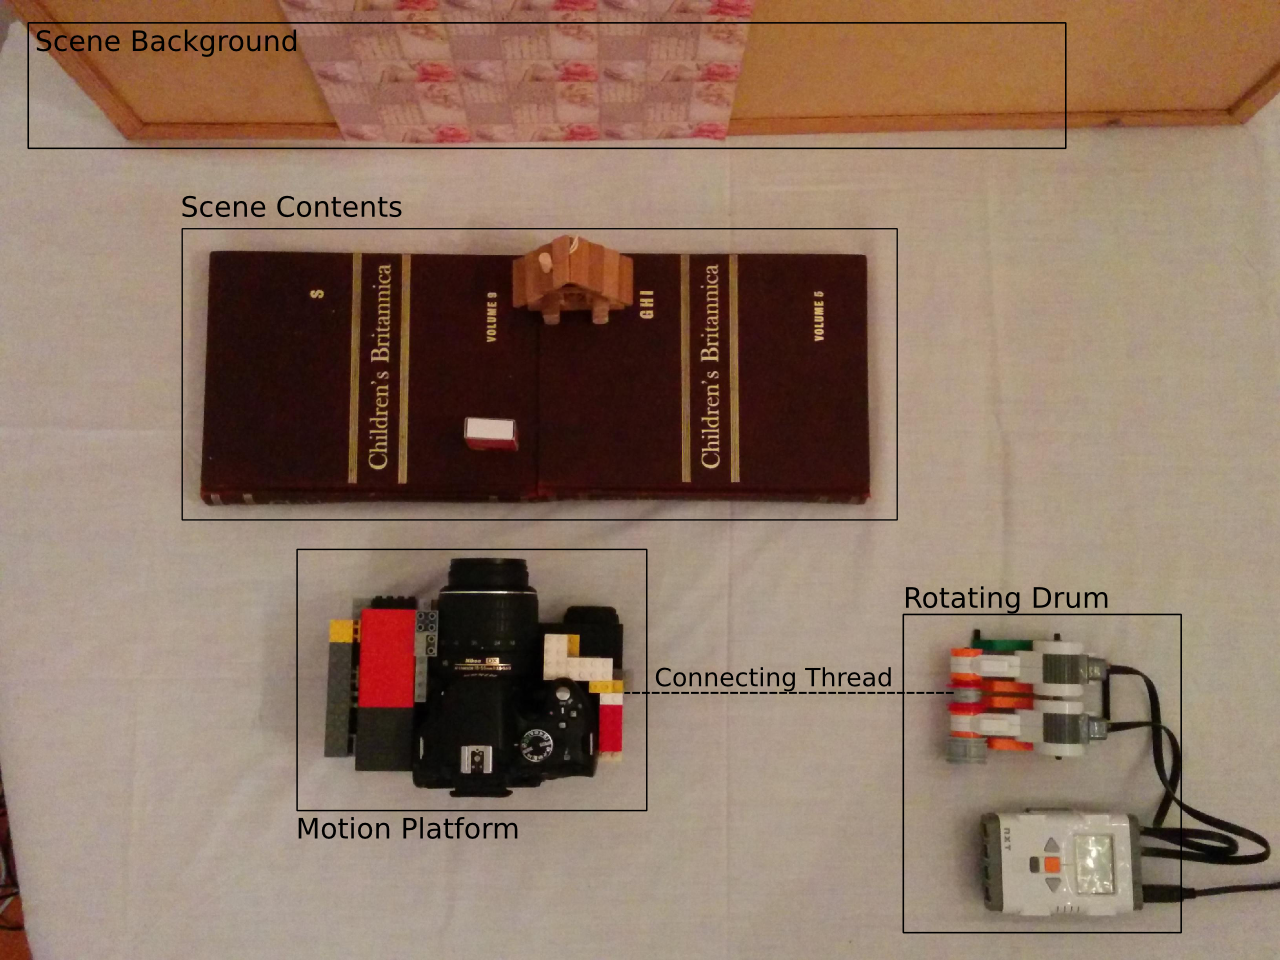
\includegraphics[width=\textwidth]{scene_contents}
\caption[Experimental scene layout]{Experimental scene layout, shown from above}
\label{fig:scene_description}
\end{figure}


\section{Image Capture}
\label{sec:image_capture}

A Lytro camera with firmware version 1.2.2 was used for the light field photography.
The Lytro camera was configured using the following settings.

\begin{table}[h]
\centering
\caption{Lytro Camera Settings}
\label{tab:lytro_settings}
\begin{tabular}{r | l}
Zoom & 1.0 \\
Creative Mode & Off \\
ND Filter & Off \\
ISO Sensitivity & Auto \\
Shutter Speed & As Required \\
Shutter Delay & 10s \\
\end{tabular}
\end{table}

The shutter delay was set to 10s to allow the motion platform to reach a stable velocity.
Once the camera countdown was started, the motion platform was commanded to move for a set distance at a set velocity.
In several cases multiple attempts were required to get the entire scene within the narrow Lytro field of view.

The captured images were transfered to an computer using the standard Lytro Desktop companion software, version 3.1.1 for Mac.
A late 2011 model Apple Mac Book Air running OSX 10.9.3 was used for image processing and version 0.2 of the Light Field Toolbox \cite{dansereau2013toolbox} was used for light field manipulation and processing in Matlab.
The image decoding process used by the LF toolbox is described in \cite{dansereau2013decoding}.

Lytro .lfp files were converted to raw image files and metadata files using the python-lfp-reader Python scripts (version 0.2) \cite{esfahbod2013python}, as per the Matlab LF Toolbox instructions.

The original purpose of the DSLR camera was to capture ground-truth sharp images for comparison with the light field images.
Unfortunately due to the shallow depth range used in the experiment the DSLR images were unable to focus on all objects in the scene.
The DSLR was left in-place for all images to ensure the motion platform velocity calculations were correct, however the actual DSLR images were not used at all.

\section{Image Processing and Deconvolution}
\label{sec:image_processing_and_deconvolution}

The raw image files were read using the Matlab LF Toolbox and the Lytro depth maps were extracted from the Lytro desktop software image database.

Camera velocity was measured using the Lego Mindstorms motor encoders on the motion platform after initial calibration of the platform with a stopwatch and ruler.

The exposure time and focal length were read from the Lytro image metadata, and a scaling factor for the Lytro focal length determined experimentally.

To de-blur the light field, all possible sup-aperture slices were taken and individually de-convoled once at every scene depth using the Richardson-Lucy method, as implemented in the Matlab command 'deconvlucy'.
The de-convoled sub-aperture images were then combined, using the depth plane pixel masks.
This Matlab code for this process is fully described in Appendix XXXX.


\section{Quantitative Analysis}
\label{sec:quantitative_analysis}

Two quantitative measures were used to compare de-blurred light fields.
A \enquote*{Q-Factor} was computed to measure the increase in image sharpness and the Root-Mean-Square Error (RMSE) was estimated to measure the degree of noise amplification introduced by the de-convolution.

The Q-Factor was computed by summing absolute pixel intensities after applying a vertical Prewitt edge detection filter.
These sums were then normalised relative to the original blurred image Q-factor.
This had the effect of measuring the increase in the intensity of high-frequency components in the image.
Thus, the Q-factor we used was

\begin{equation}
Q = \frac{\sum_{x=1}^{W} \sum_{y=1}^{H}
\left| (I \ast H)(x, y) \right|
\label{eq:q_factor}}{Q_b}
\end{equation}

where $Q_b$ is the Q-Factor for the original image, $W$ and $H$ are the width and height of the image, $I$ is the de-blurred image, and is the Prewitt vertical edge detection kernel.

\begin{equation}
H = 
\begin{bmatrix}
1 & 0 & -1 \\
1 & 0 & -1 \\
1 & 0 & -1 \\
\end{bmatrix}
\label{eq:prewitt_filter}
\end{equation}

(the vertical detection kernel was used due to the presence of horizontal motion blur in the tests performed here).

This Q-factor definition had the downside of also measuring noise content.
Thus, noisy images could potentially score higher than clean, sharp images.
Without a ground truth image, a simple and well defined measure of \enquote*{image sharpness} is not easy to formulate, as evidenced by the complexity of image sharpness standards \cite{imatest2014sharpness}.
Despite this, our Q factor definition served to demonstrate the quantifiable recovery of high-frequency image content after de-blurring.

The RMSE was estimated by converting the central sub-aperture image to grayscale, then selecting a small (approximately 50x50 pixel) region known to be of constant color.
The RMSE was then computed using

\begin{equation}
R = \sqrt{ \sum_{x=1}^{W} \sum_{y=1}^{H} (I(x,y) - m)^2 }
\end{equation}

Where $W$ and $H$ are the width and height of the region respectively, $I$ is the region image and $m$ is the gray level within the region.
This metric gives an estimate of the additive noise content in the image prior to de-blurring, and an estimate of the noise (ringing and additive) in the image after de-blurring.

